%!TEX root = Thesis.tex

\section{Results \& Review}

We replicate the numerical \& analytical results of the papers of Carmichael  \& Bishop\cite{Carmichael2015}\cite{Bishop2010}, by computationally solving the master equation, mean-field methods, and monte-carlo simulations.

\subsection{Numerical}
Truncating the master equation density matrix Fock state expansion produces a finite set of coupled differential equations for the components, from which for low photon occupation expectation values in full quantum generality can be generated to high accuracy. This method does however scale incredible poorly in the system size (the number of elements in the density matrix $\propto N^2$, where N is the dimension of the system Hilbert space. The method of quantum trajectories scales much better \cite{Molmer1993} $\propto N$ by considering the wavefunction stochastically). Setting the time derivatives to zero here yields a matrix equation, which given the positive definiteness and hermiticity conditions on the density matrix yields to a Cholesky solver \cite{Press1992}. We use the Matlab and Python solvers as exposed by QuTiP \cite{Johansson2013a} and qotoolbox\cite{Tan}.For the time dependent solutions, we also use fourth order runge-kutta methods provided in both libaries.

\begin{figure}[ht]
 \includegraphics[width=0.4\textwidth]{01:03:2016 - MatlabMeanFieldvsQuantum.png}
 \caption{Comparison of mean field and fully quantum contour plots with critical points at $\frac{\Epsilon}{2}$ highlighted}\label{fig:MeanFieldvsQuantum}
\end{figure}
\begin{figure}
 \begin{minipage}{.5\linewidth}
     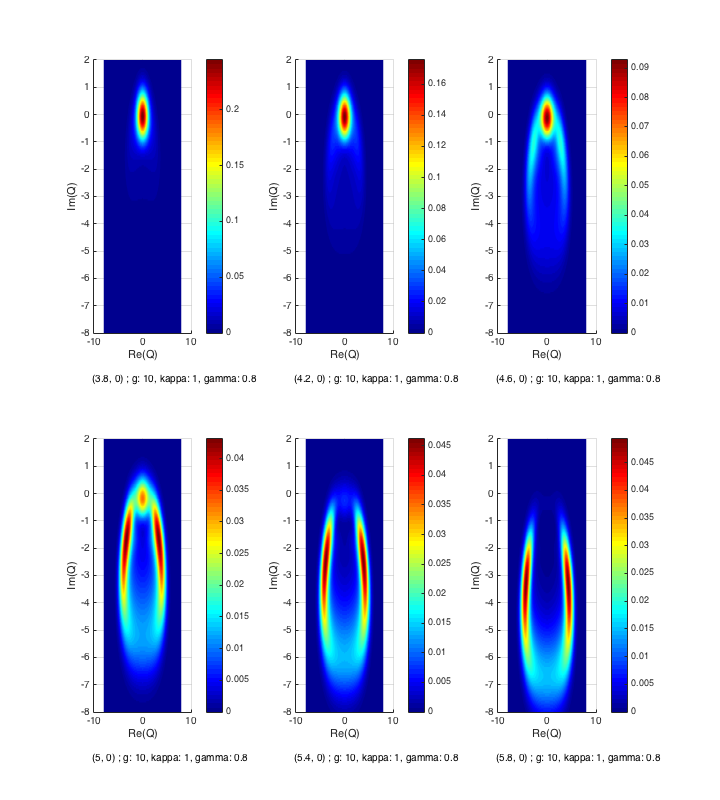
\includegraphics[width=1\textwidth]{Q-Bistability-OnResonance.png}
  \end{minipage}%
  \begin{minipage}{.5\linewidth}
      \includegraphics[width=1\textwidth]{Q-Bistability-OffResonance.png}
  \end{minipage}
  \caption{(a) Development of phase bistability in the W function for fixed detuning, with drive moving through the critical point at $\frac{\Epsilon}{2}$ \label{fig:Qbistabilities}(b) W functions with changing detuning and fixed drive. Note the probability fringes to the right connecting the peaks by spontaneous emission}
\end{figure}
\begin{figure}
 \includegraphics[width=0.5\textwidth]{01:03:2016 - MatlabCriticalSlowing.png}
  \caption{Time Dependent Solutions with g=0.5, $\kappa$ = 0.01, blue line is (0.24, 1), red line is (0.1, 1)}\label{fig:CriticalSlowing}
\end{figure}
\subsection{Analytical}

We consider the extent to which quantum fluctuations affect the dynamics by deriving an effective mean-field theory.

Taking expectation values $\langle \dot{O} \rangle = tr\{\dot{\rho} O \}$ of the operators $a, \atann, \sigma_z$ we obtain

\begin{align}
  \langle \dot{\ann} \rangle & = i(-\delta_{qd}\langle a \rangle - ig \langle \atann \rangle -i\Epsilon) -\kappa \langle a \rangle \\
  \langle \dot{\sigma_-} \rangle & = i(-\delta_{ad}\atann - ig \langle a \sigma_z \rangle) - \gamma \langle \atann \rangle \\
  \langle \dot{\sigma_z} \rangle & = -2g ( \langle \cre \sigma \rangle + \langle \ann \sigma^\dagger \rangle) - 2 \gamma \langle \sigma_z \rangle - 2 \gamma
\end{align}
we now make the assumption that all expectation values of products of operators factorize. This corresponds to the assumption that there are no correlations between different operators - this is patently non-physical, but the approximation yields equations in which the quantum fluctuation effects of these correlations are averaged out, and the qualitative behaviour remains the same to high order \cite{Jaynes1963a}. Defining $\langle \ann \rangle = \alpha, \langle \atann \rangle = \beta, \langle \sigma_z \rangle = \zeta$, setting $\delta_{cd} = \delta_{qd}$ i.e. qubit-cavity resonance, neglecting spontaneous emission $\gamma=0$ \footnote{ Interestingly, setting $\gamma$ equal to zero at this point yields different asymptotic solutions to those for the system with $\gamma$ included and set to zero in the solution \cite{Carmichael2015}}, and adiabatically eliminating the drive, we attain what are known as the optical Bloch equations
\begin{align}
  &\frac{d \alpha}{dt} = -(\kappa -i \Delta \omega) \alpha-ig \beta \label{eq:alpha}\\
  &\frac{d \beta}{dt} = i \Delta \omega \beta +ig \alpha \zeta \label{eq:beta}\\
  &\frac{d \zeta}{dt} = 2 i g(\alpha^* \beta -\alpha \beta^*)\label{eq:zeta}
\end{align}
Since the length of the pseudo-spin is conserved in the absence of dissipation (here $\kappa$ is added phenomenologically and has no mixing effect) we have also a fourth equation
\begin{equation}
  4|\beta|^2+\zeta^2 = 1 \label{eq:pseudospin}
\end{equation}
By a similar process, with the spontaneous emission parameter $\gamma$ included from the start, we obtain another set of coupled differential equations. In this case however, the length of the Bloch spin is not conserved, and the system comes to steady state inside the Bloch sphere.
